\section{Case Study 1}

The pilot case study implements the movie ticket reservation system prototype described in the outline earlier, primarily using microservices communicating with REST APIs. Representational State Transfer implies that a client requesting a resource from any service, cues the server to transfer back the current state of the resource in a standardised representation. The system design and implementation details are elaborated below.

\subsection{Design and Implementation}

\begin{figure}[H]
  \centering
  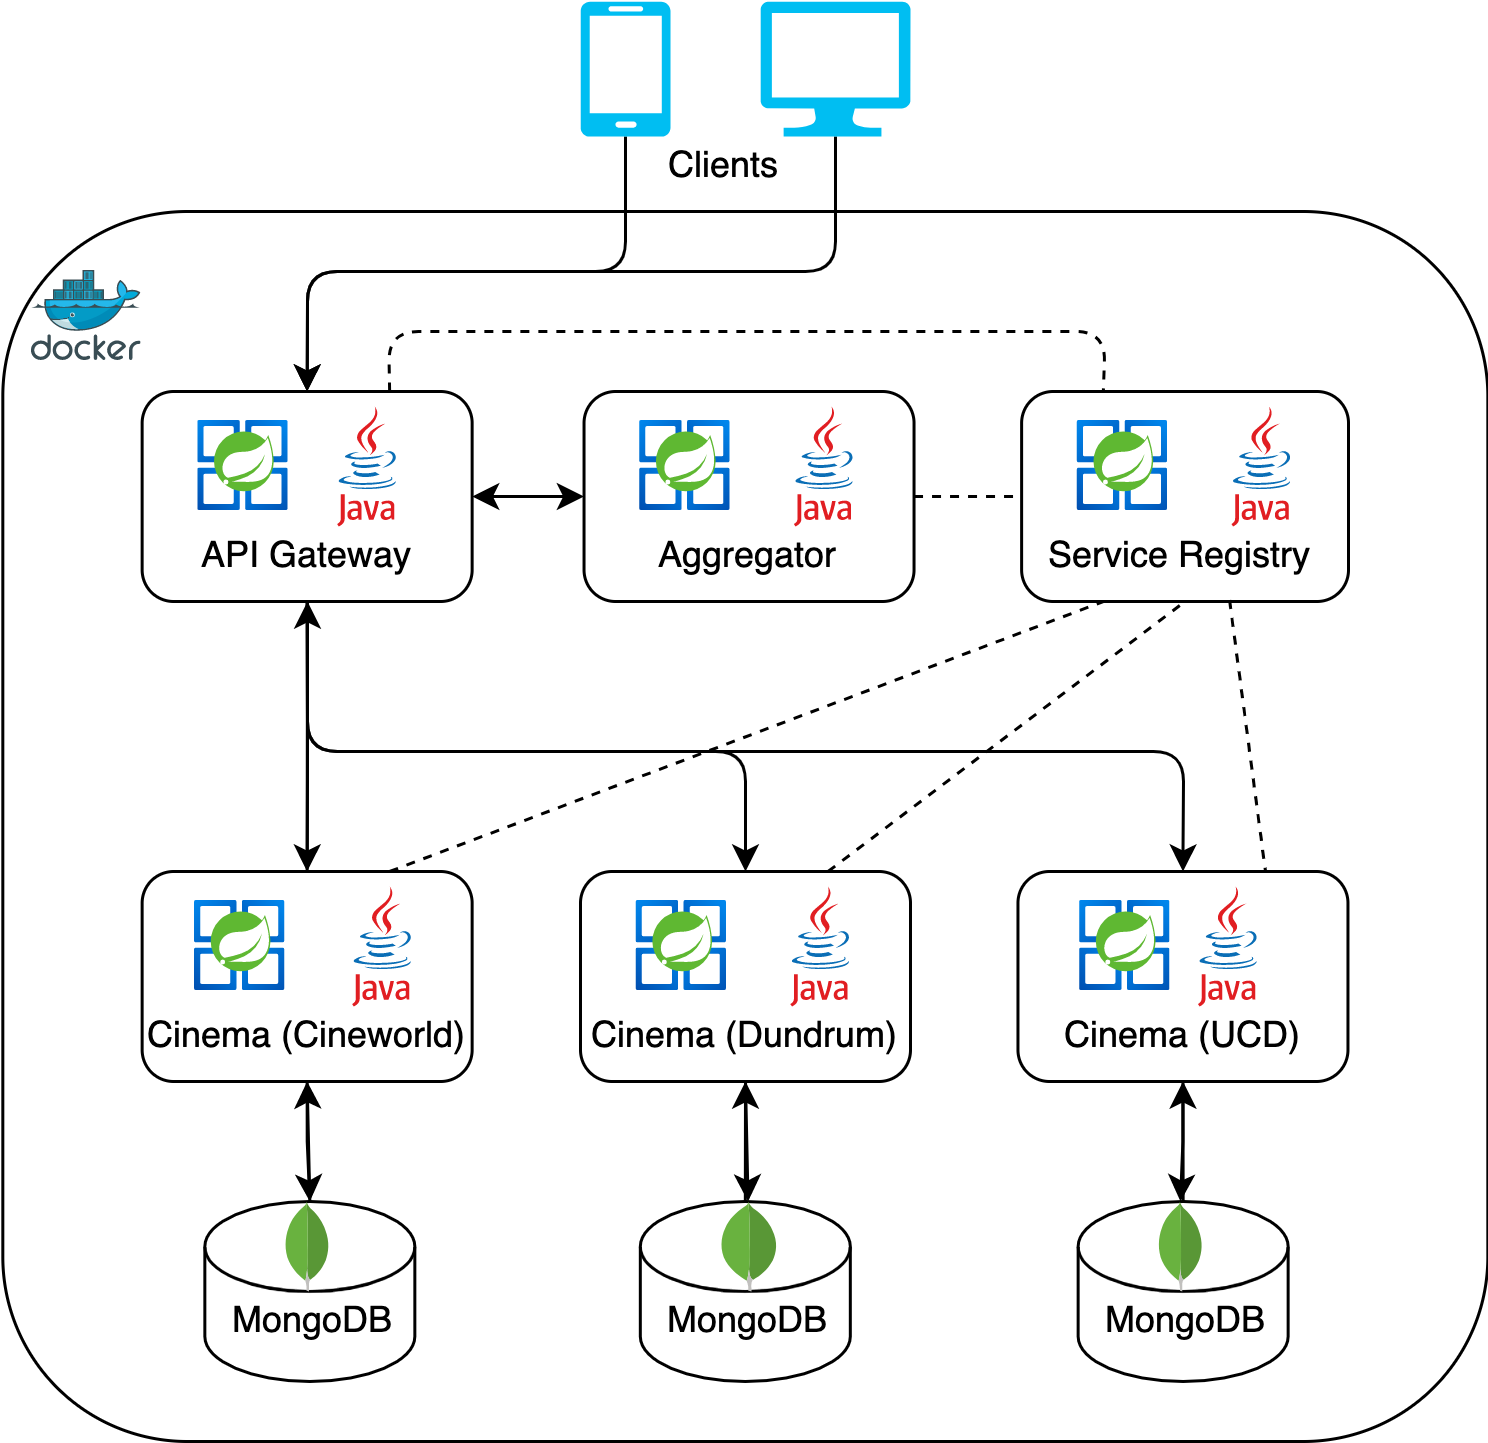
\includegraphics[width=0.6\linewidth]{./assets/diagrams/cs01-arch.png}
  \caption{System design for the first case study.}
  \label{fig:cs01-arch}
\end{figure}

The architecture diagram above (Fig. \ref{fig:cs01-arch}) depicts the organisation of the microservices involved: an API gateway service to act as an interface between clients and other services, and aggregator service to gather results, and three independent cinema services - Cineworld, Dundrum and UCD. The following microservice design patterns have been employed while developing this web application:

\subsubsection{API Gateway}

An \textit{API gateway} is one of the most fundamental and commonly used design patterns in microservice architecture. The \code{api-gateway-service} microservice offers an entry point for all clients, so that multiple services (e.g. cinemas) can be exposed, and gateway can route requests to other services as appropriate. In such situations, an API gateway relieves the clients from setting up and managing a separate endpoint for every service. It also aids the inter-service communication between microservices when required, for instance, the \code{aggregator-service} contacts the cinema services via the gateway again.

Without a gateway, any change (e.g. refactoring) in the service APIs would necessitate corresponding changes in the client code as well, which creates several development and management troubles. However, when a gateway is placed between clients and services, further consolidation or decomposition of a service would only require a simple routing change, instead of updating the client.

An added benefit of this pattern would be the ease of deployment of new versions of microservices, which can be done in parallel with existing versions, since API gateway routing would provide control over endpoints presented to clients, and flexibility over feature release strategies.

A minor variation of the API gateway pattern is called \textit{backends for frontends (BFF)}, where a separate gateway handles request routing for different kinds of clients, such as web applications, mobile applications and third part applications (e.g. IoT devices). API endpoint management in appropriate gateway services is a more focussed approach to handling routing logic for different kinds of user interfaces, with their own set of pre-requisites.

Despite its popularity and usefulness, the API gateway pattern brings with it a few issues that should be taken into consideration. For instance, it could become a bottleneck or single point of failure, if resiliency and fault tolerance measures are not put in place. Performance testing methods such as load testing should be explored to prevent failure scenarios.

In this case study, the \code{api-gateway-service} uses the Spring Cloud project to introduce a gateway in the application.

\begin{lstlisting}[language=XML, caption=Maven dependency for Spring Cloud Gateway]
  <dependency>
    <groupId>org.springframework.cloud</groupId>
    <artifactId>spring-cloud-starter-gateway</artifactId>
  </dependency>
\end{lstlisting}

The gateway is configured using the module's \code{application.yml} resource file, which Spring Boot can access to set up all the routing logic supported by the application. From a performance perspective, an API gateway provides several benefits, such as options to set up request authentication, rate-limiting to prevent service over-use and DDoS attacks, monitoring and analytics endpoints (using Spring Boot Actuator), reducing latency by serving cached responses, as well as load balancing. A very simple gateway configuration example is shown below. The \code{lb://} prefix in \code{uri:} makes use of Spring Cloud Gateway's built-in load balancer, to provide round robin client-side load balancing features during calls to other microservices. A 503 Service Unavailable Error is returned when a service cannot be found, which is more appropriate than a basic Java exception stack trace shown when using \code{http://} or \code{https://} prefixes instead.

\begin{lstlisting}[caption=Sample Spring Cloud Gateway configuration]
  spring:
    cloud:
      gateway:
        routes:
        - id: myRoute
          uri: lb://service
          predicates:
          - Path=/service/**
\end{lstlisting}

Spring Cloud Gateway paves the way for discussion on the next two design patterns: \textit{circuit breaker} and \textit{client-side service discovery}, thanks to the integrations available to simplify configuration and maintenance.


\subsubsection{Circuit Breaker}

\subsubsection{Client-side Service Discovery}

\subsubsection{Aggregator}

\subsubsection{Externalised Configuration}

Externalised configuration is a cross-cutting concerns design pattern, that is especially useful in separating changeable application properties from the business logic. Spring Boot has built-in support for processing external configuration from various sources, such as Java properties files, YAML files, environment variables, and command-line arguments. The values set by the developer for such properties are injected into Spring beans \footnote{\url{https://www.baeldung.com/spring-bean}} using the \code{@Value} annotation (among other alternatives).

Shown below are the environment variable settings for Cineworld's cinema service in the first case study's Docker Compose file.
\begin{lstlisting}[caption=Snippet from \code{docker-compose.yml}]
  cinema-cineworld-service:
    ...
    environment:
      - SERVER_PORT=8082
      - EUREKA_SERVER=eureka-server
      - DATABASE_HOST=mongodb
      - DATABASE_PORT=27017
    ...
\end{lstlisting}

Using the above environment variables, Spring Boot then sets the application properties. Externalising configuration also allows the development team to maintain all properties in one place (say the Docker Compose file) such that any required changes will only need to be made in that file, instead of searching for every occurrence of the property in the application source code.

\begin{lstlisting}[caption=Snippet from \code{cinema-cineworld-service} \code{application.yml} file]
  server:
    servlet:
      context-path: /cinema/cineworld
    port: $\dollar${SERVER_PORT}
  spring:
    application:
      name: cinema-cineworld-service
    data:
      mongodb:
        database: cinema-cineworld
        host: $\dollar${DATABASE_HOST:mongodb}:$\dollar${DATABASE_PORT:27017}
  eureka:
    ...
    client:
      ...
      serviceUrl:
        defaultZone: http://$\dollar${EUREKA_SERVER:eureka-server}:$\dollar${EUREKA_PORT:8761}/eureka/
\end{lstlisting}

\subsubsection{Database per Service}

\subsubsection{Service Instance per Container}

The services have been built as a multi-module Maven project, each having an independent Dockerfile for deployment.


\subsection{Evaluation}
